\section{Planification}
\label{sec:chronologie}

	Cette séparation des tâches nous a permis de réaliser un diagramme de Gantt du projet, avec des ressources affectées pour chaque tâche. Retranscrire exactement le diagramme de Gantt ne rendrait pas celui-ci très lisible, nous avons donc réalisé grâce à l'outil disponible sous Microsoft Project une frise chronologique qui reprend dans les grandes lignes ce dernier. Celui-ci est cependant disponible en annexe pour voir la liste entière de toutes les tâches du projet.

	Tel qu'annoncé dans les rapports précédents, l'effectif de notre groupe pour la phase de conception et pour la phase de développement se voit réduit, puisqu'il ne restera plus que Marlène, Alexandre et Romain; les autres membres du groupe partant en semestre à l'étranger. Nous avons planifié l'estimation des tâches en prenant en compte cette réduction des ressources. Nous avons considéré 8h de travail par semaine par membre du projet (hormis les semaines réservées au projet, la semaine de partiel et les semaines de vacances où les horaires de travail sont différents), ceci sans compter les heures des réunions prévues chaque mercredi. Cela représente donc 24h de travail effectif par semaine normale.

	Nous avons fixé la date de commencement de la phase de pré-développement au 16 janvier; les deux semaines précédentes étant consacrées aux révisions des partiels. La date de livraison finale est fixée au 27 mai (dernier délai). Cette livraison comprendra tous les rapports, les transparents des soutenances, les sources commentées, la documentation, les tests, une procédure d'installation et une machine virtuelle contenant la plateforme installée ainsi que tous les outils nécessaires. Ainsi, la durée entre le début de la phase de conception et la livraison finale est de 18 semaines.

	Les livraisons intermédiaires, quant à elles, sont déterminées à partir du temps de développement des fonctionnalités spécifiques à celles-ci. Ces dates, présentes dans la chronologie que vous pouvez retrouver plus bas, pourront donc légèrement varier suivant les retours que l'on recevra à chaque livraison. 

	D'un côté, un document Microsoft Project, qui a permis la génération du diagramme de Gantt, de la planification et de la chronologie, sera mis à jour au fur et à mesure du développement pour suivre celui-ci dans le temps et s'assurer que les possibles retards n'impactent pas sur les livraisons ou sur le développement des fonctionnalités. D'un autre côté, et ce depuis le début du projet, nous avons un modèle sur Google sheet fourni par Yoann Royer qui nous permet de suivre pas-à-pas les tâches. Le principe est simple; les tâches sont insérées et listées dans le document. Celles-ci peuvent être : Assignée, En cours ou Terminée. Cet état est mis au fur et à mesure; d'abord par le chef de projet (qui assigne les tâches), puis par le propriétaire de la tâche. Chaque tâche dispose d'une ligne dans le document, et chaque colonne représente un jour. Il est possible de rentrer dans celles-ci le temps passé sur la tâche pour chaque jour. Enfin une colonne en fin de semaine résume le temps passé sur cette tâche. Si elle n'est pas terminée, la personne chargée de la réaliser dispose d'une colonne 'Reste à faire' lui permettant d'estimer le temps qu'il pense nécessaire pour réaliser la tâche.

	Les trois membres restants seront chef de projet à tour de rôle. Marlène occupera ce rôle du 16 janvier au 28 février, Alexandre du 29 février au 17 avril, et enfin Romain du 18 avril jusqu'à la fin du projet, le 26 mai. Marlène s'occupe aussi de vérifier que chaque personne rentre bien son suivi de temps chaque semaine.

	Vis-à-vis des risques, lors de la planification des tâches et des durées sur Microsoft, nous avons déterminé un taux d'utilisation de chaque membre de 90\%, et avec la planification actuelle, nous prévoyons d'être capable de fournir la livraison finale le 17 mai. Cela nous laisse une dizaine de jours pour compenser tout retard possible.



	\begin{figure}[H]
        \centering
        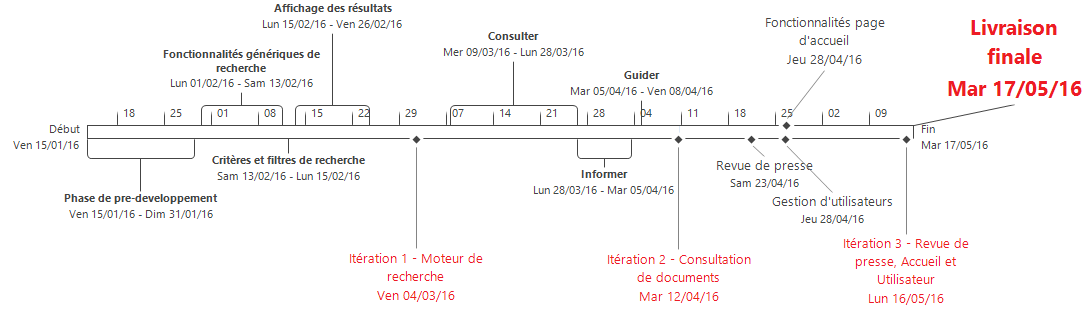
\includegraphics[width=1.3\textwidth, angle=90]{figure/frise.png}
            \caption{Frise chronologique représentant l'ensemble de la planification}
            \label{fig:frise}
    \end{figure}
